\documentclass[border=0.5cm]{standalone}
\usepackage{amsmath,amsfonts}
\usepackage{tikz}
\begin{document}


			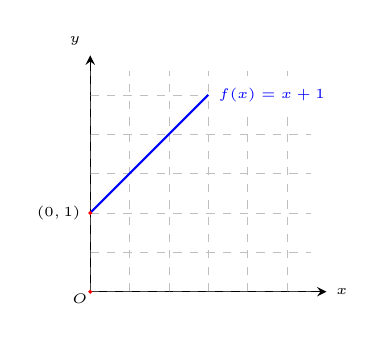
\begin{tikzpicture}
				%% estilos
				\tikzstyle{coor} = [line width=0.5pt,>=stealth,->]
				\tikzstyle{format}=[font=\tiny]
				\tikzstyle{graph} = [thick,blue]
				\tikzstyle{point} = [color=red,fill=red]
				%%%%

			%% coordenadas
			\draw[coor](0,0)--(3,0) node[format,right]{$x$};
			\draw[coor](0,0)--(0,3) node[format,above left]{$y$};
			%%%%

				%% Grid
				\draw[help lines,dashed,step=0.5cm,opacity=0.5] (0,0) grid (2.8,2.8);
				%%%%
				
			%% funcion
			\draw[graph] plot[domain=0:1.5,samples=50] ({\x},{\x+1}) node[format,right,fill=white]{$f(x)=x+1$};
			%%%%

			%%puntos
			\coordinate (O) at (0,0);
			\draw[point](O)circle(0.5pt) node[black,below left=-2.5pt, format]{$O$};
			\coordinate (A) at (0,1);
			\draw[point](A)circle(0.5pt) node[black,left,format]{$(0,1)$};
			%%%%
		\end{tikzpicture} 	
\end{document}
